\documentclass{article}

\usepackage[spanish]{babel}

\usepackage[letterpaper,top=2cm,bottom=2cm,left=3cm,right=3cm,marginparwidth=1.75cm]{geometry}

\usepackage{listings}
\usepackage{graphicx}
\usepackage[colorlinks=true, allcolors=blue]{hyperref}

\title{Proyecto Integrador}
\author{Sebastian Marines Alvarez - A01383056}

\begin{document}
\maketitle

\begin{abstract}
Se desarrolló el juego del ahorcado como proyecto final de la materia TC1028.1. El código del proyecto se puede encontrar en el \href{https://github.com/sebastianmarines/TC1028.1}{repositorio} de GitHub
\end{abstract}

\section{Introducción}
El juego depende de 2 librerías externas para funcionar: \textbf{Pillow} para la carga y manejo de imágenes y \textbf{Tk} para la interfaz gráfica.

El objetivo de este juego es que las personas puedan mantener su mente activa y ejercitar sus capacidades cognitivas a través de los juegos.

Conforme las personas se van acercando a la vejes, muchas palabras se olvidan y se espera que este juego ayude a mejorar los recuerdos de estas palabras.\\

\begin{figure}[h]
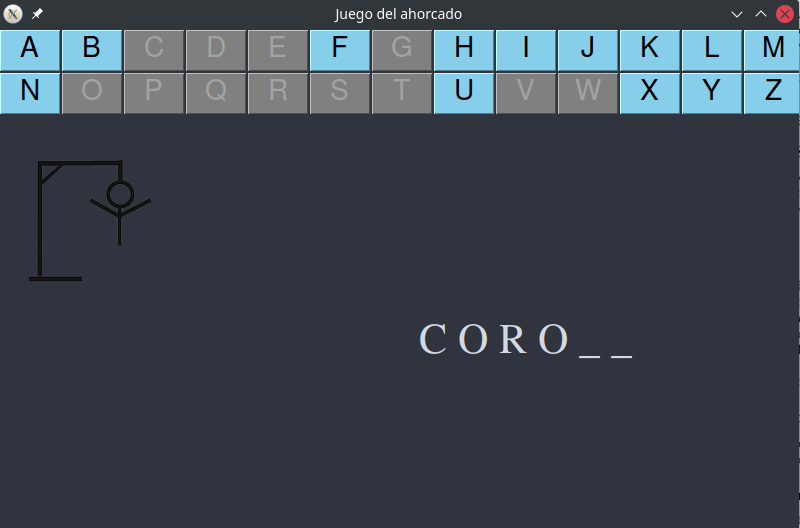
\includegraphics[width=\textwidth]{demo.png}
\caption{Demo del juego}
\label{fig:demo}
\end{figure}

\section{Funcionamiento}

\subsection{Objetivo}

El objetivo de el juego es adivinar una palabra aleatoria en menos de 11 intentos. Cada vez que se hace click en una letra cuenta como un intento.

\subsection{Descripción}

Al iniciar el juego se lee una palabra del archivo que contiene las palabras y se elige una palabra aleatoria, se muestran espacios vacíos que representan cada letra de la palabra y el usuario puede usar los botones de letras que se encuentran en la parte superior para adivinar las letras que contiene.

Si palabra a adivinar contiene la letra que el usuario ingresó se muestra la letra o letras en la palabra; si la palabra no contiene la letra se le resta una ``vida`` al usuario y se dibuja otra parte del ahorcado.

El usuario comienza el juego con 11 vidas, y una vez que se queda sin vidas se muestra la palabra que tenia que adivinar y se le da la opción de volver a jugar como se muestra en la figura \ref{fig:lose}

\begin{figure}[h]
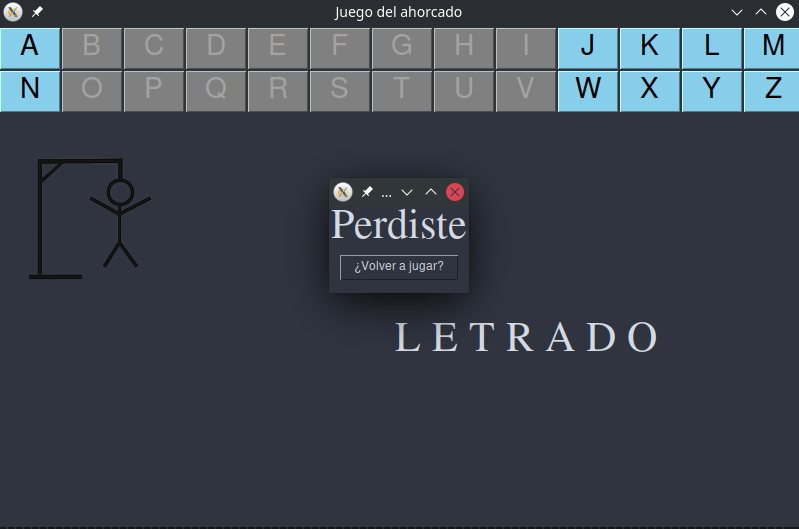
\includegraphics[width=\textwidth]{lose.png}
\caption{Pantalla que se muestra al usuario cuando pierde}
\label{fig:lose}
\end{figure}

Si el usuario adivina toda la palabra antes de que se le acaben los intentos se muestra una pantalla donde se indica que ganó y un botón con la opción de jugar de nuevo como se muestra en la figura \ref{fig:win}

\begin{figure}[h]
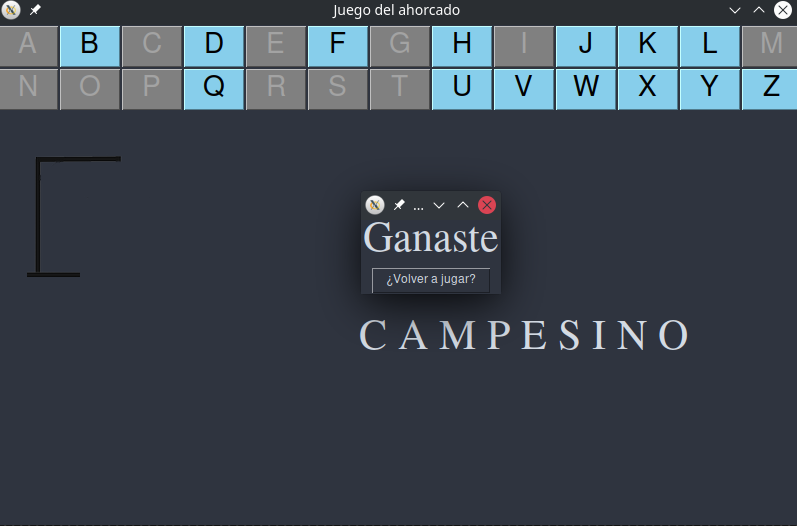
\includegraphics[width=\textwidth]{win}
\caption{Pantalla que se muestra al usuario cuando gana}
\label{fig:win}
\end{figure}

El juego termina una vez que el usuario adivina la palabra o se queda sin intentos

\section{Dificultades}

Uno de los problemas que se tuvo al elaborar el proyecto fue determinar las librerías que se usarían, ya que quería depender lo menos posible de librerías que no estuvieran incluidas en la librería estándar de Python. Al final opté por usar \textbf{Tk} como interfaz gráfica, ya que viene incluida con la mayoría de las instalaciones de Python.

Otra problema que se presentó fue conseguir una fuente de palabras en español, ya que la mayoría de los recursos de este tipo se encuentran en inglés. 
Opté por escribir un \href{https://github.com/sebastianmarines/TC1028.1/blob/master/scraper.exs}{script} que extrajera palabras de una pagina de internet y las guardara en un archivo para que pudieran ser usadas por el juego.

\end{document}